\documentclass[preprint,12pt,a4paper]{elsarticle}
%DIF LATEXDIFF DIFFERENCE FILE
%DIF DEL ../v_1/bruteforce.tex   Sat Aug  1 21:39:39 2026
%DIF ADD bruteforce.tex          Sat Aug  1 21:39:39 2026

\usepackage{amssymb}
\usepackage{float}
\usepackage{listings}
\PassOptionsToPackage{hyphens}{url}
\usepackage{hyperref}
\usepackage{xcolor}
\usepackage{lineno}
\setlength{\parindent}{0pt}
\emergencystretch=3em
\sloppy
\lstdefinestyle{mystyle}{
    basicstyle        = \ttfamily\footnotesize,
    breakatwhitespace = false,
    breaklines        = true,
    captionpos        = b,
    keepspaces        = true,
    numbersep         = 5pt,
    showspaces        = false,
    showstringspaces  = false,
    showtabs          = false,
    keywordstyle      = \color{blue},
    stringstyle       = \color{green},
    commentstyle      = \color{red}\ttfamily
}
\lstset{style=mystyle}

\restylefloat{table}
\journal{SoftwareX}
 %DIF > 
% --------------------------------------------------------------------------- %DIF > 
% TODO(authors) -- resolve before resubmission: \datarepo must resolve publicly. %DIF > 
% The URL below returned HTTP 404 on 2026-08-01 (the local clone's remote is %DIF > 
% git@github.com:lpawela/omni-bench), which is exactly what reviewers 2 and 3 %DIF > 
% flagged.  Publish the repository at this address (ideally pointing at an %DIF > 
% immutable tag) or update the macro to wherever it ends up living. %DIF > 
% --------------------------------------------------------------------------- %DIF > 
\newcommand{\datarepo}{https://github.com/euro-hpc-pl/omni-bench} %DIF > 
\newcommand{\datareponame}{\texttt{euro-hpc-pl/omni-bench}} %DIF > 
 %DIF > 
% TODO(authors): confirm which CUDA Toolkit version was used on the H100 cluster %DIF > 
% for the reported measurements (CI builds and tests with 12.5), then replace the %DIF > 
% macro body below with the plain version string and drop the red marker. %DIF > 
\newcommand{\cudameas}{\textcolor{red}{12.5 (to be confirmed)}} %DIF > 
%DIF PREAMBLE EXTENSION ADDED BY LATEXDIFF
%DIF UNDERLINE PREAMBLE %DIF PREAMBLE
\RequirePackage[normalem]{ulem} %DIF PREAMBLE
\RequirePackage{color}\definecolor{RED}{rgb}{1,0,0}\definecolor{BLUE}{rgb}{0,0,1} %DIF PREAMBLE
\providecommand{\DIFaddtex}[1]{{\protect\color{blue}\uwave{#1}}} %DIF PREAMBLE
\providecommand{\DIFdeltex}[1]{{\protect\color{red}\sout{#1}}}                      %DIF PREAMBLE
%DIF SAFE PREAMBLE %DIF PREAMBLE
\providecommand{\DIFaddbegin}{} %DIF PREAMBLE
\providecommand{\DIFaddend}{} %DIF PREAMBLE
\providecommand{\DIFdelbegin}{} %DIF PREAMBLE
\providecommand{\DIFdelend}{} %DIF PREAMBLE
\providecommand{\DIFmodbegin}{} %DIF PREAMBLE
\providecommand{\DIFmodend}{} %DIF PREAMBLE
%DIF FLOATSAFE PREAMBLE %DIF PREAMBLE
\providecommand{\DIFaddFL}[1]{\DIFadd{#1}} %DIF PREAMBLE
\providecommand{\DIFdelFL}[1]{\DIFdel{#1}} %DIF PREAMBLE
\providecommand{\DIFaddbeginFL}{} %DIF PREAMBLE
\providecommand{\DIFaddendFL}{} %DIF PREAMBLE
\providecommand{\DIFdelbeginFL}{} %DIF PREAMBLE
\providecommand{\DIFdelendFL}{} %DIF PREAMBLE
%DIF HYPERREF PREAMBLE %DIF PREAMBLE
\providecommand{\DIFadd}[1]{\texorpdfstring{\DIFaddtex{#1}}{#1}} %DIF PREAMBLE
\providecommand{\DIFdel}[1]{\texorpdfstring{\DIFdeltex{#1}}{}} %DIF PREAMBLE
%DIF COLORLISTINGS PREAMBLE %DIF PREAMBLE
\RequirePackage{listings} %DIF PREAMBLE
\RequirePackage{color} %DIF PREAMBLE
\lstdefinelanguage{DIFcode}{ %DIF PREAMBLE
%DIF DIFCODE_UNDERLINE %DIF PREAMBLE
  moredelim=[il][\color{red}\sout]{\%DIF\ <\ }, %DIF PREAMBLE
  moredelim=[il][\color{blue}\uwave]{\%DIF\ >\ } %DIF PREAMBLE
} %DIF PREAMBLE
\lstdefinestyle{DIFverbatimstyle}{ %DIF PREAMBLE
	language=DIFcode, %DIF PREAMBLE
	basicstyle=\ttfamily, %DIF PREAMBLE
	columns=fullflexible, %DIF PREAMBLE
	keepspaces=true %DIF PREAMBLE
} %DIF PREAMBLE
\lstnewenvironment{DIFverbatim}{\lstset{style=DIFverbatimstyle}}{} %DIF PREAMBLE
\lstnewenvironment{DIFverbatim*}{\lstset{style=DIFverbatimstyle,showspaces=true}}{} %DIF PREAMBLE
%DIF END PREAMBLE EXTENSION ADDED BY LATEXDIFF

\begin{document}

\begin{frontmatter}

\title{Omnisolver: An extensible interface to Ising spin--glass and QUBO
solvers \DIFdelbegin \DIFdel{: adding }\DIFdelend \DIFaddbegin \DIFadd{--- }\DIFaddend a \DIFaddbegin \DIFadd{numerically stabilized, }\DIFaddend distributed GPU \DIFdelbegin \DIFdel{brute-force }\DIFdelend \DIFaddbegin \DIFadd{exhaustive-search }\DIFaddend plugin}

\author[1]{Konrad Ja\l{}owiecki}
\cortext[cor1]{Corresponding author}
\author[2,3]{Jakub Paw{\l}owski}
\author[1,2]{Bart{\l}omiej Gardas}
\author[1,2]{{\L}ukasz Pawela\corref{cor1}}
\ead{lpawela@iitis.pl}

\address[1]{Institute of Theoretical and Applied Informatics, Polish Academy
of Sciences, Ba{\l}tycka 5, 44-100 Gliwice, Poland}

\address[2]{Quantumz.io Sp. z o. o., Pu{\l}awska 12/3, 02-566 Warsaw, Poland}

\address[3]{Institute of Theoretical Physics, Faculty of Fundamental Problems
of Technology, Wroc{\l}aw University of Science and Technology,
50-370 Wroc{\l}aw, Poland}

\begin{abstract}
This software update \DIFdelbegin \DIFdel{extends
}\DIFdelend \DIFaddbegin \DIFadd{matures }\texttt{\DIFadd{omnisolver-bruteforce}}\DIFadd{, the exhaustive-search
plugin of }\DIFaddend Omnisolver~\cite{jalowiecki2021omnisolver}\DIFdelbegin \DIFdel{with
}\texttt{\DIFdel{omnisolver-bruteforce}}%DIFAUXCMD
\DIFdel{, a first-class plugin for exact exhaustive
search }\DIFdelend \DIFaddbegin \DIFadd{, into a released and
API-stable backend for exact ground-state certification }\DIFaddend of QUBO and Ising
instances on CUDA-enabled GPUs. \DIFdelbegin \DIFdel{The update
contributes three components: packaging of the single-GPU brute-force
kernel of ~\mbox{%DIFAUXCMD
\cite{jalowiecki2021brute} }\hskip0pt%DIFAUXCMD
as a first-class Omnisolver plugin with a uniform Python and
CLI interface, a }\DIFdelend \DIFaddbegin \DIFadd{Throughout, $N$ denotes the number of binary
variables of an instance (equivalently, the number of Ising spins), so that
exhaustive search enumerates all $2^{N}$ configurations. The plugin itself,
together with a preliminary multi-GPU benchmark, was already announced in the
original publication; the present update contributes a released }\DIFaddend Ray-based
distributed \DIFdelbegin \DIFdel{framework }\DIFdelend \DIFaddbegin \DIFadd{sampler }\DIFaddend that splits the search into $2^{k}$ fixed-variable
subproblems\DIFdelbegin \DIFdel{and }\DIFdelend \DIFaddbegin \DIFadd{, }\DIFaddend dispatches them across multiple GPUs and hosts \DIFdelbegin \DIFdel{, with a controller that gathers and merges partial results,
and }\DIFdelend \DIFaddbegin \DIFadd{and merges the
partial results on a controller; }\DIFaddend numerical stabilization of the fast
\texttt{float32} ground-state path through compensated incremental updates,
periodic exact energy re-anchoring \DIFdelbegin \DIFdel{, }\DIFdelend and best-buffer refresh\DIFdelbegin \DIFdel{. Stabilization activates automatically for $N \geq 40$ }\DIFdelend \DIFaddbegin \DIFadd{, enabled
automatically for per-kernel subproblems of at least $40$ variables and }\DIFaddend leaving
the public sampler API \DIFdelbegin \DIFdel{is unchanged}\DIFdelend \DIFaddbegin \DIFadd{unchanged; and 64-bit-safe enumeration bookkeeping that
lifts the reachable problem size beyond the original single-GPU regime}\DIFaddend . On dense
random Ising instances we \DIFdelbegin \DIFdel{measure exhaustive solve times }\DIFdelend \DIFaddbegin \DIFadd{certify exhaustive ground states }\DIFaddend up to $N=60$ on
$8\times$ NVIDIA H100 (96\,GB) GPUs, reaching $\approx\!3.15$ days at $N=60$\DIFdelbegin \DIFdel{in close
}\DIFdelend \DIFaddbegin \DIFadd{, in
}\DIFaddend agreement with the empirical $t_{N+1}=2\,t_N$ doubling rule \DIFdelbegin \DIFdel{, with }\DIFdelend \DIFaddbegin \DIFadd{to within $0.3\%$.
Measured against the single-GPU sampler on identical instances, }\DIFaddend the distributed
sampler \DIFdelbegin \DIFdel{reaching the full $\approx\!8\times$ speedup over a
single H100 from
$N\!\gtrsim\!44$ onwards. The plugin thereby serves as a
practical ground-truth oracle for state-of-the-art classical heuristics such
as the }\DIFdelend \DIFaddbegin \DIFadd{crosses over between $N=40$ and $N=42$, attains $93\%$ parallel
efficiency at $N=48$ and saturates at the ideal $8\times$ speedup from
$N\!\gtrsim\!52$. The certified optima serve as ground truth for a }\DIFaddend Simulated
Bifurcation Machine \DIFaddbegin \DIFadd{run on the same instances, which is found to recover the
exact ground-state configuration in every case tested}\DIFaddend .
\end{abstract}

\begin{keyword}
QUBO \sep Ising \sep spin glass \sep exhaustive search \sep GPU \sep
\DIFaddbegin \DIFadd{parallel efficiency }\sep \DIFaddend Omnisolver plugin \sep software update
\end{keyword}

\end{frontmatter}

\section*{Refers to}
K.~Ja\l{}owiecki, {\L}.~Pawela, ``Omnisolver: An extensible interface to Ising
spin--glass and QUBO solvers,'' \emph{SoftwareX} \textbf{24}, 101559 (2023).
DOI: \url{https://doi.org/10.1016/j.softx.2023.101559}.

\section*{Metadata}
\label{metadata}

%DIF >  TODO(authors): C1/C2 -- the repository at tag 0.0.5 still contains no LICENSE
%DIF >  file (GitHub license endpoint returns 404, pyproject.toml declares no license,
%DIF >  PyPI shows no license classifier), so C3 below is not yet backed by the code.
%DIF >  Reviewer 3 checked this.  Add LICENSE (Apache-2.0), the license field and
%DIF >  classifier in pyproject.toml, `include LICENSE` in MANIFEST.in and per-file
%DIF >  license headers, cut release 0.0.6 and bump C1/C2/S1/S2 accordingly.
%DIF >  TODO(authors): C7 -- the linked documentation redirects to version 0.0.3, has
%DIF >  no content about this plugin and contains dead links; the plugin's own
%DIF >  mkdocs.yml references docs/userguide.md and docs/plugins.md, which do not
%DIF >  exist, so its build is broken.  Either publish the plugin documentation and
%DIF >  point C7/S6 at it, or point C7 at a page that is actually useful.
\begin{table}[H]
\setlength{\tabcolsep}{4pt}
\begin{tabular}{|l|p{5.6cm}|p{6.4cm}|}
\hline
\textbf{Nr.} & \textbf{Code metadata description} & \textbf{Value} \\
\hline
C1 & Current code version & 0.0.5 \\
\hline
C2 & Permanent link to code/repository used for this code version &
\url{https://github.com/euro-hpc-pl/omnisolver-bruteforce/releases/tag/0.0.5} \\
\hline
C3 & Legal Code License & Apache License 2.0 \\
\hline
C4 & Code versioning system used & git \\
\hline
C5 & Software code languages, tools, and services used & Python, C++, Cython,
CUDA, Ray \\
\hline
C6 & Compilation requirements, operating environments \& dependencies & Linux
\DIFdelbeginFL \DIFdelFL{,
CUDA Toolkit }\DIFdelendFL \DIFaddbeginFL \DIFaddFL{(x86-64) with a CUDA-capable NVIDIA GPU; CUDA Toolkit (builds and tests in
continuous integration use 12.5; the measurements reported here were obtained
with \cudameas)}\DIFaddendFL , \texttt{Python >= 3.10}, \texttt{omnisolver >= 0.0.4},
\texttt{dimod \DIFdelbeginFL %DIFDELCMD < \MBLOCKRIGHTBRACE%%%
\DIFdelFL{, }\texttt{\DIFdelFL{numba}}%DIFAUXCMD
\DIFdelFL{, }\DIFdelendFL \DIFaddbeginFL \DIFaddFL{~= 0.12}}\DIFaddFL{, }\DIFaddendFL \texttt{\DIFdelbeginFL \DIFdelFL{numpy}\DIFdelendFL \DIFaddbeginFL \DIFaddFL{numba ~= 0.58}\DIFaddendFL }, \texttt{\DIFdelbeginFL \DIFdelFL{ray}\DIFdelendFL \DIFaddbeginFL \DIFaddFL{numpy ~= 2.0}\DIFaddendFL }\DIFaddbeginFL \DIFaddFL{;
}\texttt{\DIFaddFL{ray >= 2.9}} \DIFaddFL{is additionally required by the distributed sampler }\DIFaddendFL \\
\hline
C7 & Link to developer documentation/manual &
\url{https://euro-hpc-pl.github.io/omnisolver/} \\
\hline
C8 & Support email for questions & \verb|lpawela@iitis.pl| \\
\hline
\end{tabular}
\caption{Code metadata}
\label{codeMetadata}
\end{table}

\DIFaddbegin \begin{table}[H]
\setlength{\tabcolsep}{4pt}
\begin{tabular}{|l|p{5.6cm}|p{6.4cm}|}
\hline
\textbf{\DIFaddFL{Nr.}} & \textbf{\DIFaddFL{(Executable) software metadata description}} &
\textbf{\DIFaddFL{Value}} \\
\hline
\DIFaddFL{S1 }& \DIFaddFL{Current software version }& \DIFaddFL{0.0.5 }\\
\hline
\DIFaddFL{S2 }& \DIFaddFL{Permanent link to executables of this version }&
\url{https://pypi.org/project/omnisolver-bruteforce/0.0.5/}\DIFaddFL{; the distribution is
a source archive, so the CUDA extension is compiled at installation time against
the CUDA Toolkit available on the target machine }\\
\hline
\DIFaddFL{S3 }& \DIFaddFL{Legal Software License }& \DIFaddFL{Apache License 2.0 }\\
\hline
\DIFaddFL{S4 }& \DIFaddFL{Computing platforms/Operating Systems }& \DIFaddFL{Linux (x86-64) with a CUDA-capable
NVIDIA GPU; the reported measurements were performed on NVIDIA H100 96\,GB
(compute capability }\texttt{\DIFaddFL{sm\_90}}\DIFaddFL{) }\\
\hline
\DIFaddFL{S5 }& \DIFaddFL{Installation requirements \& dependencies }& \DIFaddFL{CUDA Toolkit (continuous
integration: 12.5; measurements: \cudameas), }\texttt{\DIFaddFL{Python >= 3.10}}\DIFaddFL{,
}\texttt{\DIFaddFL{omnisolver >= 0.0.4}}\DIFaddFL{, }\texttt{\DIFaddFL{dimod}}\DIFaddFL{, }\texttt{\DIFaddFL{numba}}\DIFaddFL{, }\texttt{\DIFaddFL{numpy}}\DIFaddFL{;
}\texttt{\DIFaddFL{ray >= 2.9}} \DIFaddFL{for the distributed sampler; at build time additionally
}\texttt{\DIFaddFL{cython}} \DIFaddFL{and }\texttt{\DIFaddFL{setuptools-cuda}} \\
\hline
\DIFaddFL{S6 }& \DIFaddFL{Link to user manual }& \url{https://euro-hpc-pl.github.io/omnisolver/} \\
\hline
\DIFaddFL{S7 }& \DIFaddFL{Support email for questions }& {\color{blue}%DIFAUXCMD
\verb|lpawela@iitis.pl| %
}%DIFAUXCMD
\\
\hline
\end{tabular}
\caption{\DIFaddFL{Software metadata}}
\label{softwareMetadata}
\end{table}

\DIFaddend \linenumbers

\section{Description of the software update}
\label{sec:description}

Omnisolver~\cite{jalowiecki2021omnisolver} is a plugin-based framework that
exposes a uniform Python and command-line interface to QUBO/Ising solvers,
integrated with \texttt{dimod}. \DIFaddbegin \DIFadd{A solver is contributed as an independent
package that registers itself through an entry point and ships a small
specification file, from which the framework derives the command-line interface
and the input/output handling; solvers can therefore be interchanged without
touching the surrounding workflow. }\DIFaddend The original publication established the
framework \DIFdelbegin \DIFdel{and }\DIFdelend \DIFaddbegin \DIFadd{together with }\DIFaddend its first plugins, \DIFdelbegin \DIFdel{for example, the Parallel Tempering solver}\DIFdelend \DIFaddbegin \DIFadd{among them a parallel-tempering
sampler and the exhaustive-search plugin discussed here}\DIFaddend . This update \DIFdelbegin \DIFdel{introduces
}\texttt{\DIFdel{omnisolver-bruteforce}}%DIFAUXCMD
\DIFdel{, a dedicated plugin that promotes a previously
stand-alone single-GPU exhaustive solver~\mbox{%DIFAUXCMD
\cite{jalowiecki2021brute} }\hskip0pt%DIFAUXCMD
to a first-class Omnisolver component,
adds }\DIFdelend \DIFaddbegin \DIFadd{concerns
the latter, }\texttt{\DIFadd{omnisolver-bruteforce}}\DIFadd{: it turns the plugin into a released,
API-stable certification backend, contributes a }\DIFaddend distributed multi-GPU \DIFdelbegin \DIFdel{execution
through }\DIFdelend \DIFaddbegin \DIFadd{sampler
built on }\DIFaddend Ray~\cite{DBLP:journals/corr/abs-1712-05889}, and stabilizes the
numerical behavior of its fast ground-state path.

\DIFaddbegin \DIFadd{Throughout this paper, $N$ denotes the number of binary variables of an instance
(equivalently, the number of Ising spins), so that exhaustive search enumerates
all $2^{N}$ configurations. The remaining quantities used below are the
parameters exposed by the plugin's samplers: }\texttt{\DIFadd{num\_states}} \DIFadd{is the number
of lowest-energy states to be returned, }\texttt{\DIFadd{num\_fixed\_vars}}\DIFadd{\,$=k$ is the
number of variables whose values are frozen in order to define independent
subproblems in the distributed sampler, and }\texttt{\DIFadd{suffix\_size}} \DIFadd{is the number
of variables forming the enumeration suffix, i.e.\ $2^{\texttt{suffix\_size}}$
configurations are resident in the GPU working set at a time and the search
sweeps $2^{N-\texttt{suffix\_size}}$ such chunks. The parameters
}\texttt{\DIFadd{grid\_size}}\DIFadd{, }\texttt{\DIFadd{block\_size}}\DIFadd{, }\texttt{\DIFadd{num\_steps\_per\_kernel}} \DIFadd{and
}\texttt{\DIFadd{partial\_diff\_buffer\_depth}} \DIFadd{control the CUDA launch geometry, the
number of chunks processed per kernel launch and the depth of the
incremental-energy buffers, respectively.
}

\DIFaddend \paragraph{Purpose of an exhaustive solver in Omnisolver}
An exhaustive backend provides \emph{certified} reference \DIFaddbegin \DIFadd{solutions}\DIFaddend , i.e.\DIFdelbegin \DIFdel{lowest-energy, solutions }\DIFdelend \DIFaddbegin \DIFadd{\
configurations of provably lowest energy, }\DIFaddend for QUBO/Ising instances. Such
ground-truth answers are essential for
benchmarking approximate or heuristic methods, for verifying NISQ-oriented
workflows~\cite{preskill2018quantum}, and for assessing claims of quantum
runtime advantage. In recent years, the latter point has become especially
critical in the community, with many studies relying on metrics that
explicitly depend on the ground-state energy, such as the \emph{optimality gap}.
For example, in recent comparative studies of runtime
advantage~\cite{tuziemski2026limits} and of the quantum-classical scaling
gap~\cite{pawlowski2025closing}, quantum resources were benchmarked against the
Simulated Bifurcation Machine
(SBM)~\cite{goto2016bifurcation,goto2019combinatorial,goto2021high,pawlowski2026sbqa},
the current state-of-the-art classical heuristic for dense QUBO/Ising problems.
Such results rely on the ability to certify the true optimum on representative
instances, which is precisely what an exhaustive GPU solver provides.

\paragraph{Architecture}
The plugin \DIFdelbegin \DIFdel{introduced by this software update }\DIFdelend exposes two sampler classes: \texttt{BruteforceGPUSampler}
(single-node, single-GPU) and \texttt{DistributedBruteforceGPUSampler}
(multi-GPU/multi-node via Ray). The distributed sampler fixes
\texttt{num\_fixed\_vars}\,$=k$ variables and enumerates all $2^{k}$ fixed
assignments\DIFdelbegin \DIFdel{, each of which becomes a }\DIFdelend \DIFaddbegin \DIFadd{; each assignment becomes an independent }\DIFaddend subproblem with $N-k$
unfixed variables, \DIFaddbegin \DIFadd{dispatched as a Ray task and }\DIFaddend solved by the GPU kernel on a
worker. Partial solutions are \DIFaddbegin \DIFadd{collected and }\DIFaddend merged on the controller node. \DIFaddbegin \DIFadd{Both
samplers accept SPIN and BINARY models: a SPIN model is converted to its BINARY
equivalent, solved as a QUBO and converted back, so the QUBO and Ising code
paths coincide up to a host-side transformation performed outside the measured
region. }\DIFaddend As a practical guideline, the single-GPU sampler \DIFdelbegin \DIFdel{is }\DIFdelend \DIFaddbegin \DIFadd{remains }\DIFaddend the right
choice \DIFdelbegin \DIFdel{while one device has both the memory budget and a }\DIFdelend \DIFaddbegin \DIFadd{as long as a single device has sufficient memory and the expected
}\DIFaddend wall-clock time \DIFdelbegin \DIFdel{within reason for the chosen problem size}\DIFdelend \DIFaddbegin \DIFadd{is acceptable}\DIFaddend ; beyond that point \DIFdelbegin \DIFdel{, }\DIFdelend the distributed sampler
amortizes the work by powers of two in the number of workers. On our hardware \DIFdelbegin \DIFdel{, }\DIFdelend it
crosses the break-even region between $N=40$ and $N=42$ (see
Fig.~\ref{fig:runtimes} \DIFaddbegin \DIFadd{and Table~\ref{tab:efficiency}}\DIFaddend ), and from
\DIFdelbegin \DIFdel{$N\!\gtrsim\!44$ it reaches }\DIFdelend \DIFaddbegin \DIFadd{$N\!\gtrsim\!52$ it attains }\DIFaddend the full $\approx\!8\times$ speedup expected from
the 8-GPU pool, \DIFdelbegin \DIFdel{with }\DIFdelend \DIFaddbegin \DIFadd{once }\DIFaddend Ray-scheduling and kernel-launch overheads \DIFaddbegin \DIFadd{are }\DIFaddend amortized
over the per-subproblem \DIFdelbegin \DIFdel{compute}\DIFdelend \DIFaddbegin \DIFadd{computation}\DIFaddend . Performance-critical kernels are
implemented in CUDA/C++ and exposed to Python via Cython; the
\texttt{num\_states=1} fast path operates in \texttt{float32} to maximize GPU
throughput, with the stabilization mechanisms described below compensating for
the resulting roundoff.

\paragraph{Relation to the \DIFaddbegin \DIFadd{original publication and to the }\DIFaddend predecessor \DIFdelbegin \DIFdel{single-GPU }\DIFdelend solver}
\DIFdelbegin \DIFdel{On }\DIFdelend \DIFaddbegin \DIFadd{The exhaustive-search plugin is not new, and we state its provenance
explicitly. The original Omnisolver
publication~\mbox{%DIFAUXCMD
\cite{jalowiecki2021omnisolver} }\hskip0pt%DIFAUXCMD
already lists
}\texttt{\DIFadd{omnisolver-bruteforce}} \DIFadd{among the available plugins, notes that it can be
accelerated on CUDA-enabled GPUs, describes it as usable for instances of up to
about $50$ variables, and reports a preliminary benchmark of the GPU sampler on
$1$, $2$, $4$ and $8$ NVIDIA A100 GPUs. Its computational core goes back further
still, to the stand-alone single-GPU solver of~\mbox{%DIFAUXCMD
\cite{jalowiecki2021brute}}\hskip0pt%DIFAUXCMD
: on
}\DIFaddend instances that fit a single device \DIFdelbegin \DIFdel{, the }\DIFdelend \DIFaddbegin \DIFadd{the present }\DIFaddend kernel is API-compatible with
\DIFdelbegin \DIFdel{the original solver of~\mbox{%DIFAUXCMD
\cite{jalowiecki2021brute} }\hskip0pt%DIFAUXCMD
}\DIFdelend \DIFaddbegin \DIFadd{that solver }\DIFaddend and reproduces its per-state throughput within measurement noise\DIFdelbegin \DIFdel{; the present }\DIFdelend \DIFaddbegin \DIFadd{, so
this }\DIFaddend update does not re-benchmark the single-device axis but inherits its
performance envelope\DIFdelbegin \DIFdel{and adds, on top of it, the stabilization patches and the distributed
controller}\DIFdelend \DIFaddbegin \DIFadd{. What the update contributes is therefore not the existence
of a GPU-accelerated or multi-GPU exhaustive search, but its maturation into a
dependable certification backend, as detailed next}\DIFaddend .

\paragraph{Update contributions}
\begin{itemize}
    \item \textbf{\DIFdelbegin \DIFdel{First-class Omnisolver plugin}\DIFdelend \DIFaddbegin \DIFadd{Released, API-stable distributed sampler}\DIFaddend }: the \DIFdelbegin \DIFdel{brute-force kernel is available through Omnisolver's plugin mechanism with a uniform Python and
    CLI interface, returning }\DIFdelend \DIFaddbegin \DIFadd{multi-GPU code
    path is now a documented, versioned public class
    (}\texttt{\DIFadd{DistributedBruteforceGPUSampler}}\DIFadd{, tagged }\texttt{\DIFadd{0.0.5}} \DIFadd{and
    published on PyPI) rather than the unreleased code behind the preliminary
    benchmark of~\mbox{%DIFAUXCMD
\cite{jalowiecki2021omnisolver}}\hskip0pt%DIFAUXCMD
, and it returns a
    }\DIFaddend \texttt{dimod.SampleSet} \DIFdelbegin \DIFdel{with runtime metadata .
    }%DIFDELCMD < \item %%%
\item%DIFAUXCMD
\textbf{\DIFdel{Distributed multi-GPU execution}} %DIFAUXCMD
\DIFdel{via a Ray-based fixed-variable
    decomposition, enabling exhaustive search at sizes infeasible on a single
    device within a practical time-frame}\DIFdelend \DIFaddbegin \DIFadd{carrying runtime metadata through the same plugin
    and CLI mechanism as any other Omnisolver sampler}\DIFaddend .
    \item \textbf{Stabilized fast ground-state path}: compensated incremental
    updates, periodic exact energy re-anchoring \DIFdelbegin \DIFdel{, and best-buffer refresh }\DIFdelend \DIFaddbegin \DIFadd{and a final refresh of the
    best-state buffer }\DIFaddend eliminate the \texttt{float32} drift previously observed
    \DIFdelbegin \DIFdel{for $N \geq 40$
    }\DIFdelend in the \texttt{num\_states=1} mode. Stabilization \DIFdelbegin \DIFdel{activates automatically
    ;
    the }\DIFdelend \DIFaddbegin \DIFadd{is enabled automatically
    whenever the size seen by the kernel is at least $40$ variables, that is for
    $N-k \geq 40$ in distributed runs; the public }\DIFaddend API is unchanged.
    \item \textbf{Hardening for large-$N$ enumeration}: 64-bit-safe bit
    operations and kernel-step bookkeeping \DIFdelbegin \DIFdel{support spin configurations of
    }\DIFdelend \DIFaddbegin \DIFadd{make the enumeration correct for
    configuration }\DIFaddend sizes well beyond the original single-GPU regime.
    \item \DIFaddbegin \textbf{\DIFadd{Certification reach and scaling evidence}}\DIFadd{: measurements are
    extended from the $N\approx 50$ of~\mbox{%DIFAUXCMD
\cite{jalowiecki2021omnisolver} }\hskip0pt%DIFAUXCMD
to
    $N=60$, i.e.\ by three orders of magnitude in enumerated configurations, and
    are accompanied by an explicit strong-scaling efficiency analysis
    (Table~\ref{tab:efficiency}) and by an end-to-end verification of the
    returned optima.
    }\item \DIFaddend \textbf{Extended validation}: GPU tests cross-check energies against
    from-scratch exact recomputation and against \texttt{dimod.ExactSolver} on
    \DIFdelbegin \DIFdel{tractable instances }\DIFdelend \DIFaddbegin \DIFadd{instances small enough for CPU enumeration; at benchmark scale, the returned
    configurations are additionally re-verified outside the plugin by a
    from-scratch }\texttt{\DIFadd{float64}} \DIFadd{energy recomputation and cross-checked against
    an independent heuristic solver}\DIFaddend .
\end{itemize}

\paragraph{Performance}
Figure~\ref{fig:runtimes} reports wall-clock solve times of both sampler modes on
all-to-all random Ising instances with $J_{ij},h_i\sim \mathcal{U}[-1,1]$ i.i.d.,
generated by the benchmark script \texttt{code/bf.py} \DIFdelbegin \DIFdel{from }\DIFdelend \DIFaddbegin \DIFadd{of }\DIFaddend the article repository
(one instance per size, fixed seed \DIFdelbegin \DIFdel{); }\DIFdelend \DIFaddbegin \DIFadd{$42$) and }\DIFaddend measured on a local
in-house cluster of $8\times$ NVIDIA H100 (96\,GB) GPUs (two nodes, 4 GPUs per
node, interconnected by standard Ethernet). The single-GPU sampler was run on one
of the same H100s \DIFdelbegin \DIFdel{, }\DIFdelend \DIFaddbegin \DIFadd{and }\DIFaddend the distributed sampler on all eight\DIFaddbegin \DIFadd{, with $k=3$ so that
the $2^{3}=8$ subproblems map one-to-one onto the available GPUs; both modes used
}\texttt{\DIFadd{suffix\_size}}\DIFadd{\,$=23$ and }\texttt{\DIFadd{num\_states}}\DIFadd{\,$=1$}\DIFaddend .
\DIFaddbegin 

\DIFadd{Reported times measure the solve phase only. For the single-GPU sampler the timer
brackets the CUDA search itself, excluding host-side assembly of the QUBO matrix
and decoding of the returned configurations; for the distributed sampler it
brackets subproblem dispatch and the collection of all partial results on the
controller, excluding the final merge of those partial results, which is
discussed separately below. Both exclusions are polynomial in $N$ and negligible
at the sizes reported here, but they matter for the extrapolations discussed
further on.
}

\DIFaddend The $O(2^N)$ doubling per added spin is the dominant feature \DIFdelbegin \DIFdel{on }\DIFdelend \DIFaddbegin \DIFadd{of }\DIFaddend both curves and
is \DIFdelbegin \DIFdel{clean already }\DIFdelend \DIFaddbegin \DIFadd{already evident }\DIFaddend at $N=40$ on the single-GPU axis\DIFdelbegin \DIFdel{; the }\DIFdelend \DIFaddbegin \DIFadd{: the measured single-GPU
times grow by a factor of $2.001$--$2.002$ per added variable over the whole
range $N=42,\dots,54$. The }\DIFaddend distributed curve flattens out for $N \lesssim 44$\DIFaddbegin \DIFadd{,
}\DIFaddend because timings are dominated there by kernel-launch and Ray-scheduling overhead\DIFdelbegin \DIFdel{. The distributed sampler crosses below the single-GPU sampler
between $N=40$ }\DIFdelend \DIFaddbegin \DIFadd{,
}\DIFaddend and \DIFdelbegin \DIFdel{$N=42$,
and reaches the full $\approx\!8\times$ speedup
(matching the 8-GPU pool) from
$N\!\gtrsim\!44$ }\DIFdelend \DIFaddbegin \DIFadd{settles onto the same asymptotic slope ($2.001$--$2.003$ per variable) from
$N=52$ }\DIFaddend onwards. The largest measured size, $N=60$ in the distributed mode, takes
$\approx\!272{,}300$ s ($\approx 3.15$ days), within $0.3\%$ of the
doubling-rule extrapolation from $N=58$ ($2^{2}\!\times\!67{,}900 \approx
271{,}600$ s); this empirically confirms the $t_{N+1}=2\,t_N$ rule across the
measured range. We use the same rule to project the single-GPU sampler (measured
up to $N=54$) to $N=60$ along the dashed extension in Fig.~\ref{fig:runtimes}:
the projected single-GPU wall-clock at $N=60$ is $\approx\!2.17\times 10^{6}$ s
($\approx\!25$ days), about $8.0\times$ the measured 8-GPU time at the same size
and consistent with linear strong scaling. The same rule places $N=64$ at
$\approx\!50$ days on the 8-GPU pool. Constant-factor deviations from exact
doubling (kernel-launch overhead, host/device transfer, Ray scheduling) can shift
the absolute numbers by at most a few percent but not the asymptotic scaling.

\paragraph{\DIFdelbegin \DIFdel{Scaling outlook on larger allocations}%DIFDELCMD < \MBLOCKRIGHTBRACE
%DIFDELCMD < %%%
\DIFdel{The fixed-variable decomposition is embarrassingly }\DIFdelend \DIFaddbegin \DIFadd{Strong scaling and }\DIFaddend parallel \DIFaddbegin \DIFadd{efficiency}}
\DIFadd{Because both samplers were run on the same instances, the two curves of
Fig.~\ref{fig:runtimes} can be paired size by size into an explicit
strong-scaling measurement, reported in Table~\ref{tab:efficiency} in terms of
the speedup $S=t_1/t_8$ and the parallel efficiency $E=S/8$. Below the crossover
the decomposition is dominated by fixed overheads: at $N=40$ the eight-way split
is in fact $2.1\times$ }\emph{\DIFadd{slower}} \DIFadd{than a single GPU, which is why the
single-GPU sampler remains the appropriate choice whenever one device suffices.
Efficiency then rises steeply, from $43\%$ at $N=44$ through $75\%$ at $N=46$ and
$93\%$ at $N=48$, and saturates at the ideal value from $N=52$ on, where the
per-subproblem computation dwarfs dispatch and launch overheads. The marginal
excess over unity at $N=54$ ($E=100.1\%$) is within the run-to-run variability of
these single-run timings and should be read as ideal scaling rather than as
superlinear speedup. This behavior is the expected signature of an
embarrassingly parallel decomposition whose fixed cost per subproblem is
independent of $N$: the eight-GPU pool becomes fully efficient exactly once
$2^{N-k}$-configuration subproblems are large enough to amortize that cost.
}

\begin{table}[H]
\centering
\begin{tabular}{|r|r|r|r|r|}
\hline
\DIFaddFL{$N$ }& \DIFaddFL{$t_1$ }[\DIFaddFL{s}] & \DIFaddFL{$t_8$ }[\DIFaddFL{s}] & \DIFaddFL{$S=t_1/t_8$ }& \DIFaddFL{$E=S/8$ }\\
\hline
\DIFaddFL{40 }& \DIFaddFL{2.74      }& \DIFaddFL{5.68     }& \DIFaddFL{0.48 }& \DIFaddFL{6\% }\\
\DIFaddFL{42 }& \DIFaddFL{8.20      }& \DIFaddFL{6.52     }& \DIFaddFL{1.26 }& \DIFaddFL{16\% }\\
\DIFaddFL{44 }& \DIFaddFL{32.83     }& \DIFaddFL{9.48     }& \DIFaddFL{3.46 }& \DIFaddFL{43\% }\\
\DIFaddFL{46 }& \DIFaddFL{131.54    }& \DIFaddFL{21.90    }& \DIFaddFL{6.01 }& \DIFaddFL{75\% }\\
\DIFaddFL{48 }& \DIFaddFL{527.07    }& \DIFaddFL{71.17    }& \DIFaddFL{7.41 }& \DIFaddFL{93\% }\\
\DIFaddFL{50 }& \DIFaddFL{2112.29   }& \DIFaddFL{268.90   }& \DIFaddFL{7.86 }& \DIFaddFL{98\% }\\
\DIFaddFL{52 }& \DIFaddFL{8458.17   }& \DIFaddFL{1060.68  }& \DIFaddFL{7.97 }& \DIFaddFL{99.7\% }\\
\DIFaddFL{54 }& \DIFaddFL{33912.27  }& \DIFaddFL{4235.25  }& \DIFaddFL{8.01 }& \DIFaddFL{100.1\% }\\
\hline
\end{tabular}
\caption{\DIFaddFL{Strong-scaling speedup and parallel efficiency of the distributed
sampler ($t_8$, $8\times$ H100, $k=3$) relative to the single-GPU sampler
($t_1$, one H100 of the same cluster) on identical instances; the timings are the
measured points of Fig.~\ref{fig:runtimes}. Efficiency stays below unity for
$N \lesssim 46$ because kernel-launch and Ray-scheduling overheads are not yet
amortized, exceeds $90\%$ from $N=48$ and saturates at the ideal value from
$N=52$ on. The value at $N=54$ marginally exceeds unity, which is within the
variability of these single-run timings.}}
\label{tab:efficiency}
\end{table}

\paragraph{\DIFadd{Controller cost and the limits of the decomposition}}
\DIFadd{The search phase itself involves no inter-worker communication}\DIFaddend : each of the
\DIFdelbegin \DIFdel{$2^k$ fixed assignments defines an independent GPU subproblem, with no
inter-worker communication during the search and only a trivial merge step
on the controller}\DIFdelend \DIFaddbegin \DIFadd{$2^{k}$ subproblems is an independent Ray task that fixes its own variables, runs
the CUDA search over the remaining $N-k$ and returns only the requested
}\texttt{\DIFadd{num\_states}} \DIFadd{samples. The single point of centralization is the
controller, which retrieves the $2^{k}$ partial sample sets and merges them into
one. In the released implementation this merge is a sequential concatenation
followed by a truncation, and the partial results are retrieved one object
reference at a time, so its cost grows linearly in the number of subproblems,
$O(2^{k})$, rather than logarithmically as a tree reduction would. At the eight
subproblems used here the merge amounts to eight single-sample transfers and is
immeasurably small next to a search lasting hours to days; it is also, as noted
above, outside the reported timings. It is nevertheless the component that
decides how far the decomposition can be pushed: at fixed $N$, incrementing $k$
halves the work of each subproblem while doubling the merge, so a break-even
point in $k$ necessarily exists, and it moves towards smaller $k$ as $N$
decreases. Replacing the sequential merge by a hierarchical reduction, which
would restore $O(k)$ behavior and remove the controller as a scaling
bottleneck, is therefore the most consequential item of future work
(Sec.~\ref{sec:conclusions}); locating the present break-even point
experimentally is the natural companion measurement, and it requires many
subproblems rather than many GPUs, since $2^{k}$ tasks are simply queued onto the
available devices.
}

\paragraph{\DIFadd{Scaling outlook on larger allocations}}
\DIFadd{Since the search phase is embarrassingly parallel, the size reachable on a larger
allocation follows from the measured 8-GPU baseline by simple proportionality,
for as long as the controller cost discussed above stays subdominant}\DIFaddend . As a
back-of-the-envelope projection, scaling \DIFdelbegin \DIFdel{our 8-GPU
baseline to $2^{16}$ GPUs , an allocation }\DIFdelend \DIFaddbegin \DIFadd{to $2^{14}=16{,}384$ GPUs --- a
partition size }\DIFaddend within reach of \DIFaddbegin \DIFadd{current }\DIFaddend leadership-class systems \DIFdelbegin \DIFdel{, }\DIFdelend \DIFaddbegin \DIFadd{--- }\DIFaddend with the
natural choice \DIFdelbegin \DIFdel{$k=16$ }\DIFdelend \DIFaddbegin \DIFadd{$k=14$ }\DIFaddend placing one subproblem per worker \DIFdelbegin \DIFdel{, }\DIFdelend would reduce $N=60$ from
$\approx\!3.15$ days to \DIFdelbegin \DIFdel{$\approx\!33$ s}\DIFdelend \DIFaddbegin \DIFadd{$\approx\!2.2$ min}\DIFaddend , and the projected $N=64$ time from
$\approx\!50$ days to \DIFdelbegin \DIFdel{$\approx\!9$ }\DIFdelend \DIFaddbegin \DIFadd{$\approx\!35$ }\DIFaddend min. Under a one-month wall-clock budget on
the same \DIFdelbegin \DIFdel{$2^{16}$-GPU }\DIFdelend allocation, the doubling rule places the limit for certifiable
exhaustive search at \DIFdelbegin \DIFdel{$N \lesssim 76$. This linear-in-GPU-count outlook is consistent
with the algorithmic structure; however, in practice, }\DIFdelend \DIFaddbegin \DIFadd{$N \lesssim 74$, comfortably within the $N \leq 64+k$ bound
imposed by the 64-bit per-worker configuration word. A hypothetical $2^{16}$-GPU
allocation, which exceeds the accelerator count of any system in operation today,
would move that limit only to $N \lesssim 76$: two additional variables for a
fourfold increase in resources is a direct consequence of the $O(2^N)$
complexity, and is the main reason we regard $N$ in the mid-seventies as a
practical ceiling for exhaustive certification rather than as a target. These
projections describe the search phase alone and should be read together with the
caveat above, since at $2^{14}$ workers the sequential merge of the current
implementation is expected to become the dominant term; }\DIFaddend controller-side merge
bandwidth, Ray scheduling overhead \DIFdelbegin \DIFdel{, }\DIFdelend and per-kernel launch latency\DIFdelbegin \DIFdel{would }\DIFdelend \DIFaddbegin \DIFadd{, rather than
the enumeration itself, would then }\DIFaddend set the true scaling ceiling\DIFdelbegin \DIFdel{, especially as $2^k$ approaches the number of
available workers}\DIFdelend .

\begin{figure}[t]
\centering
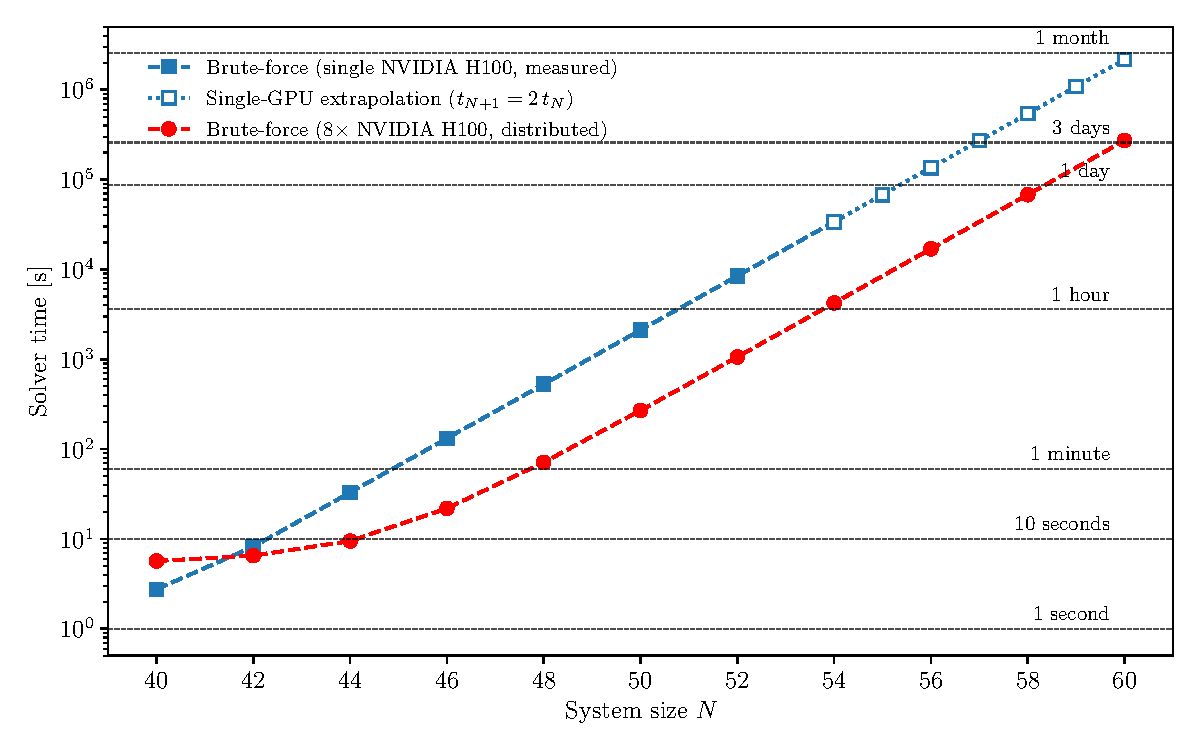
\includegraphics[width=0.95\textwidth]{distributed.pdf}
\caption{Wall-clock runtime of \texttt{omnisolver-bruteforce} on all-to-all
    random Ising instances with $J_{ij},h_i\sim \mathcal{U}[-1,1]$, measured
    on a local in-house cluster of $8\times$ NVIDIA H100 (96\,GB) GPUs (two
    nodes $\times$ 4 GPUs). Each filled marker is a single solver run on
    one fixed instance per system size $N$\DIFaddbeginFL \DIFaddFL{, where $N$ is the number of Ising
    spins, so that $2^{N}$ configurations are enumerated}\DIFaddendFL . Blue squares:
    single-GPU sampler (one of the H100s, measured for $N=40,\dots,54$). Open
    blue squares: doubling-rule extrapolation $t_{N+1}=2\,t_N$ from the largest
    measured single-GPU point to $N=60$. Red circles: distributed sampler
    on all eight GPUs \DIFaddbeginFL \DIFaddFL{with $k=3$ }\DIFaddendFL (measured for $N=40,\dots,60$). The two curves
    cross between $N=40$ and $N=42$; from \DIFdelbeginFL \DIFdelFL{$N\!\gtrsim\!44$ }\DIFdelendFL \DIFaddbeginFL \DIFaddFL{$N=52$ onwards }\DIFaddendFL the
    distributed-to-single-GPU ratio settles at the linear-scaling value
    $\approx\!8$. \DIFaddbeginFL \DIFaddFL{Table~\ref{tab:efficiency} lists the corresponding speedups
    and parallel efficiencies.}\DIFaddendFL }
\label{fig:runtimes}
\end{figure}

\paragraph{Precision of the reported energies}
Because the GPU backend operates in \texttt{float32} on the fast ground-state
path, returned energies are subject to incremental-update roundoff. We \DIFaddbegin \DIFadd{therefore
}\DIFaddend re-evaluate the energy of \DIFdelbegin \DIFdel{each }\DIFdelend \DIFaddbegin \DIFadd{every }\DIFaddend returned spin configuration from scratch in
\texttt{float64}. \DIFdelbegin \DIFdel{For the largest measured instances ($N=56,58,60$) , }\DIFdelend \DIFaddbegin \DIFadd{Across the eight single-GPU points ($N=40,\dots,54$) }\DIFaddend the
absolute deviation between \DIFdelbegin \DIFdel{reported and recomputed energies stays below $4\times 10^{-6}$ for }\DIFdelend \DIFaddbegin \DIFadd{the reported and the recomputed energy is at most
$2.4\times 10^{-5}$, and below $1\times 10^{-5}$ at all sizes but one; for the
distributed run at $N=60$ it is $4.0\times 10^{-6}$. Against }\DIFaddend energies of
magnitude $\mathcal{O}(10^{2})$ \DIFdelbegin \DIFdel{,
roughly }\DIFdelend \DIFaddbegin \DIFadd{this amounts to seven to }\DIFaddend eight significant
digits, consistent with the expected accuracy of the stabilized \texttt{float32}
accumulator. \DIFaddbegin \DIFadd{The deviation affects the reported energy }\emph{\DIFadd{value}} \DIFadd{only; the
returned configuration is an exact bit string, and its energy can be recomputed
to full }\texttt{\DIFadd{float64}} \DIFadd{accuracy by the caller at negligible cost, which is what
we do throughout and what we recommend whenever a certified numerical value, and
not merely a certified configuration, is required.
}

\DIFadd{The two samplers also provide an independent check of the decomposition itself,
since at the eight sizes where both are feasible ($N=40,\dots,54$) they solve the
same instances by different routes: a single sweep over $2^{N}$ configurations on
one device, against eight independent sweeps over $2^{N-3}$ configurations each.
They return bit-identical configurations at all eight sizes, and their reported
energies differ by at most $8.2\times 10^{-6}$, i.e.\ at the level of the
}\texttt{\DIFadd{float32}} \DIFadd{roundoff quantified above. The fixed-variable split therefore
changes the wall-clock cost of the search, not its outcome.
}

\paragraph{\DIFadd{Verification against an independent solver}}
\DIFaddend Using the same recomputation \DIFdelbegin \DIFdel{,
}\DIFdelend we cross-check \DIFdelbegin \DIFdel{an SBM }\DIFdelend \DIFaddbegin \DIFadd{a simulated-bifurcation }\DIFaddend run on the
\DIFdelbegin \DIFdel{same }\DIFdelend \DIFaddbegin \DIFadd{identical }\DIFaddend instances: a \DIFdelbegin \DIFdel{simulated bifurcation solver
running }\DIFdelend \DIFaddbegin \DIFadd{chaotic-variant, discrete simulated-bifurcation solver
(discrete and ternary update rules with automatic time-step tuning,
single-precision arithmetic, Kerr and heating terms disabled) executed }\DIFaddend on a
single H100 GPU with $2^{12}=4096$ parallel \DIFdelbegin \DIFdel{samples }\DIFdelend \DIFaddbegin \DIFadd{replicas }\DIFaddend and $3{,}000$ integration
steps, reporting the lowest-energy \DIFdelbegin \DIFdel{sample. The recomputed energies of the
brute-force and
SBM solutions agree to within $6\times 10^{-6}$, and
the returned spin
configurations are }\DIFdelend \DIFaddbegin \DIFadd{replica. On all nine instances covered by the
verification harness --- $N=40,\dots,54$ against the single-GPU sampler and
$N=60$ against the distributed one --- the configuration returned by the
simulated-bifurcation solver is }\DIFaddend bit-identical \DIFaddbegin \DIFadd{to the certified brute-force ground
state }\DIFaddend (Hamming distance $0$)\DIFdelbegin \DIFdel{at $N=56$}\DIFdelend , \DIFdelbegin \DIFdel{$58$, and $60$. On these instances, SBM }\DIFdelend \DIFaddbegin \DIFadd{and the energy it reports differs from the
}\texttt{\DIFadd{float64}} \DIFadd{recomputation of that configuration by at most $8.1\times
10^{-6}$. On this instance family the SBM therefore }\DIFaddend reaches the exact ground
state certified by exhaustive search, and the residual \DIFdelbegin \DIFdel{energy-value differences }\DIFdelend \DIFaddbegin \DIFadd{differences between the
two reported energies }\DIFaddend are explained entirely by single-precision roundoff \DIFaddbegin \DIFadd{on both
sides. This is precisely the kind of statement that cannot be made without a
certifying solver at hand, and it illustrates the intended role of the plugin}\DIFaddend .
The full verification harness (Julia driver, \DIFdelbegin \DIFdel{SBM parameters}\DIFdelend \DIFaddbegin \DIFadd{solver configuration}\DIFaddend , and the
resulting \texttt{bf\_velox\_verification\_*.csv} tables) is available in the
companion repository \DIFdelbegin %DIFDELCMD < \href{https://github.com/euro-hpc-pl/omni-bench}{%%%
\texttt{\DIFdel{euro-hpc-pl/omni-bench}}%DIFAUXCMD
\DIFdelend \DIFaddbegin \href{\datarepo}{\DIFadd{\datareponame}\DIFaddend }, together with all
\texttt{instances/*.txt} and \texttt{results/*.json} files that produced
Fig.~\ref{fig:runtimes} \DIFaddbegin \DIFadd{and Table~\ref{tab:efficiency}.
}

\paragraph{\DIFadd{Instance families, QUBO instances and other solvers}}
\DIFadd{Two properties of exhaustive search delimit what a meaningful benchmark of this
plugin can show. First, its runtime does not depend on the instance family: all
$2^{N}$ configurations are enumerated regardless of the distribution of the
coefficients, and up to the negligible bookkeeping of best-state updates the time
to solution is a function of $N$ and of the launch geometry alone. Sweeping over
coupling distributions would therefore reproduce Fig.~\ref{fig:runtimes} rather
than add information. What does depend on the family is the difficulty seen by
the heuristics that the plugin is meant to certify, so the informative extension
is to repeat the verification described above across several families --- for
instance bimodal $J_{ij}\in\{-1,+1\}$, Gaussian and sparse instances --- and to
ask whether the heuristic still recovers the certified optimum; we regard this as
the natural next application of the plugin rather than as a benchmark of the
plugin itself. Second, the QUBO and Ising paths are the same code path: both
samplers convert a SPIN model to its BINARY equivalent, solve it as a QUBO and
convert the result back, so the timings reported here are QUBO timings, the only
Ising-specific cost being an $O(N^{2})$ host-side transformation performed
outside the measured region. Correctness is cross-checked against
}\texttt{\DIFadd{dimod.ExactSolver}} \DIFadd{on instances small enough for CPU enumeration and
against from-scratch }\texttt{\DIFadd{float64}} \DIFadd{recomputation at benchmark scale; a
comparison of }\emph{\DIFadd{runtimes}} \DIFadd{against other exact solvers would add little, since
any exact method must visit an exponential number of configurations and CPU
implementations are orders of magnitude slower at the sizes considered
here~\mbox{%DIFAUXCMD
\cite{jalowiecki2021brute}}\hskip0pt%DIFAUXCMD
}\DIFaddend .

\paragraph{Limitations and intended scope}
Exhaustive enumeration scales as $O(2^N)$ irrespective of GPU count or
numerical precision: the update lowers the constant factor and removes a
\texttt{float32} drift pitfall, but it cannot change the underlying
complexity. The plugin is therefore intended as a \emph{verification and
certification backend} for QUBO/Ising research pipelines---providing
ground-truth optima against which heuristics, annealers, and NISQ-era
quantum approaches can be calibrated---rather than as a routine optimizer
for application-scale problems, where heuristic solvers such as the SBM
remain the appropriate primary tool. \DIFdelbegin \DIFdel{Concrete hard limits on }\DIFdelend \DIFaddbegin \DIFadd{The concrete hard limits of }\DIFaddend the current
implementation are: (i) the \DIFdelbegin \DIFdel{spin index }\DIFdelend \DIFaddbegin \DIFadd{per-worker spin configuration }\DIFaddend is held in a 64-bit
word, \DIFdelbegin \DIFdel{capping
the supported problem size }\DIFdelend \DIFaddbegin \DIFadd{so each subproblem is limited to $N-k \leq 64$ unfixed variables; with
$k=\texttt{num\_fixed\_vars}$ fixed variables the distributed sampler therefore
supports $N \leq 64+k$, while the single-GPU sampler is capped }\DIFaddend at $N \leq 64$\DIFaddbegin \DIFadd{,
and the caller is responsible for respecting this bound, which the release does
not yet validate}\DIFaddend ; (ii) the per-worker \texttt{suffix\_size} (the number of
variables \DIFdelbegin \DIFdel{enumerated inside one CUDA
kernel launch}\DIFdelend \DIFaddbegin \DIFadd{forming the resident enumeration chunk}\DIFaddend ) is bounded by the GPU's
L2/working-set budget and \DIFdelbegin \DIFdel{is }\DIFdelend \DIFaddbegin \DIFadd{was }\DIFaddend set to $23$ on \DIFaddbegin \DIFadd{the }\DIFaddend H100 \DIFdelbegin \DIFdel{\,/\,}\DIFdelend \DIFaddbegin \DIFadd{(}\DIFaddend 96\,GB\DIFaddbegin \DIFadd{) }\DIFaddend in our runs, so
larger $N$ must be reached by raising \texttt{num\_fixed\_vars}, not
\texttt{suffix\_size}; (iii) the \DIFaddbegin \DIFadd{numerical stabilization applies to the
}\texttt{\DIFadd{float32}} \DIFadd{ground-state path and is enabled when the size seen by the
kernel is at least $40$ variables, that is for $N-k \geq 40$ in distributed
runs, so the two smallest distributed points of Fig.~\ref{fig:runtimes} were
obtained on the unstabilized path---they nevertheless agree bit-for-bit with the
stabilized single-GPU runs at the same sizes; (iv) the }\DIFaddend projected runtimes
for $N > 60$ are back-of-the-envelope extrapolations under the empirical
$t_{N+1}=2\,t_N$ rule and may drift by a small constant factor on different
stacks\DIFaddbegin \DIFadd{; and (v) the strong-scaling measurements span two nodes and eight GPUs,
which is the extent of the hardware available to us, so the behavior of the
controller at the allocation sizes discussed above remains a projection based on
the structure of the implementation rather than a measurement}\DIFaddend . Reported runtimes
additionally depend on the hardware and software stack (GPU model, CUDA
toolkit, Ray version, interconnect), so the absolute timings in
Fig.~\ref{fig:runtimes} should be read as a hardware-specific operating
point rather than a universal guarantee.

\section{Illustrative example}
\label{sec:example}
The plugin is distributed as \texttt{omnisolver-bruteforce} on PyPI
(\texttt{pip install omnisolver-bruteforce}) and is usable either
stand-alone or through the Omnisolver CLI\DIFaddbegin \DIFadd{, under which it registers }\DIFaddend as the
\texttt{bruteforce-gpu} solver\DIFdelbegin \DIFdel{. Complete documentation and the benchmark script }\DIFdelend \DIFaddbegin \DIFadd{; the distributed sampler additionally requires
}\texttt{\DIFadd{ray}} \DIFadd{to be present in the environment. Since the distribution is a
source archive, installation compiles the CUDA extension locally and therefore
needs a CUDA Toolkit installation. The sources and the documentation of the
plugin are in the
}\href{https://github.com/euro-hpc-pl/omnisolver-bruteforce}{\DIFadd{plugin
repository}}\DIFadd{~(C2). The benchmark and plotting scripts }\DIFaddend used to produce
Fig.~\ref{fig:runtimes} \DIFdelbegin \DIFdel{are available in the }%DIFDELCMD < \href{https://github.com/euro-hpc-pl/omnisolver-bruteforce}{%%%
\DIFdel{GitHub
repository}\DIFdelend \DIFaddbegin \DIFadd{and Table~\ref{tab:efficiency} are in the article
repository, under }\texttt{\DIFadd{code/}}\DIFadd{, and read the instances, raw results and
verification tables from the companion data repository
}\href{\datarepo}{\DIFadd{\datareponame}\DIFaddend }\DIFdelbegin \DIFdel{~(C2)}\DIFdelend .

A minimal distributed-sampler invocation looks as follows:

\begin{lstlisting}[language=Python,caption={Minimal distributed brute-force example},label={lst:bf-min}]
from omnisolver.bruteforce.gpu.distributed import DistributedBruteforceGPUSampler
from dimod.serialization import coo

with open("instance.txt") as fd:
    bqm = coo.load(fd, vartype="SPIN")

sampler = DistributedBruteforceGPUSampler()
result = sampler.sample(
    bqm,
    num_states=1,
    num_fixed_vars=3,
    suffix_size=23,
    grid_size=8192,
    block_size=1024,
    partial_diff_buffer_depth=10,
    num_steps_per_kernel=8192,
)
print(result.first.energy, result.info["solve_time_in_seconds"])
\end{lstlisting}

For multi-GPU execution, Ray must be started on the head and worker
nodes (here, an 8-GPU two-node setup with 4 GPUs per node), after which the
benchmark script reproduces the curve in Fig.~\ref{fig:runtimes}:

\begin{lstlisting}[language=bash,caption={Ray startup and benchmark command used to produce Fig.~\ref{fig:runtimes}},label={lst:ray-commands}]
# Head node
ray stop --force
ray start --head --port=6379 --num-gpus=4

# Worker node
ray stop --force
ray start --address='<HEAD_NODE_IP>:6379' --num-gpus=4

# Run benchmark sweep (from the article repository root)
python code/bf.py --start 40 --stop 60 --step 2 \
                  --sampler-mode distributed --seed 42 \
                  --skip-existing
\end{lstlisting}

\section{Conclusions and outlook}
\label{sec:conclusions}
This update \DIFdelbegin \DIFdel{promotes the CUDA brute-force kernel
of~\mbox{%DIFAUXCMD
\cite{jalowiecki2021brute}}\hskip0pt%DIFAUXCMD
to a first-class Omnisolver plugin, equips it with distributed multi-GPU execution }\DIFdelend \DIFaddbegin \DIFadd{turns the exhaustive-search plugin announced
in~\mbox{%DIFAUXCMD
\cite{jalowiecki2021omnisolver}}\hskip0pt%DIFAUXCMD
, whose CUDA core originates
in~\mbox{%DIFAUXCMD
\cite{jalowiecki2021brute}}\hskip0pt%DIFAUXCMD
, into a released and API-stable certification
backend: it ships a versioned distributed sampler that executes the
fixed-variable decomposition across multiple GPUs and hosts }\DIFaddend through Ray,
\DIFdelbegin \DIFdel{and }\DIFdelend resolves the \texttt{float32} stability issue of the fast ground-state \DIFdelbegin \DIFdel{path---all
}\DIFdelend \DIFaddbegin \DIFadd{path, and
hardens the enumeration bookkeeping for large configuration sizes---all }\DIFaddend without
changing the public sampler API. On dense random Ising instances we now certify
exhaustive ground states up to $N=60$ on $8\times$ H100 GPUs, empirically
confirming the $t_{N+1}=2\,t_N$ doubling rule across the measured range\DIFaddbegin \DIFadd{, and we
quantify the strong scaling of the decomposition, which reaches $93\%$ parallel
efficiency at $N=48$ and the ideal $8\times$ speedup from $N=52$ on}\DIFaddend . Natural
next steps are: (i) \DIFaddbegin \DIFadd{replacing the controller-side merge by a hierarchical
reduction so that the algorithm scales cleanly to $2^k$ workers with large $k$,
together with a direct measurement of the present controller cost as a function
of the number of subproblems, which does not require a large GPU allocation;
(ii) complementing the strong-scaling data with a weak-scaling sweep in which
$k$ grows with the number of devices so that the per-GPU work $2^{N-k}$ stays
fixed; (iii) }\DIFaddend exposing the re-anchoring cadence and \DIFaddbegin \DIFadd{the }\DIFaddend compensated-update mode
as user-tunable knobs for instance families where the default policy is
suboptimal; (\DIFdelbegin \DIFdel{ii) replacing the
controller-side merge by a hierarchical reduction so the algorithm scales
cleanly to $2^k$ workers with $k$ approaching the system size}\DIFdelend \DIFaddbegin \DIFadd{iv) extending the certified verification of heuristic solvers from
one instance family to several, which is where certified optima are most
valuable}\DIFaddend ; and (\DIFdelbegin \DIFdel{iii}\DIFdelend \DIFaddbegin \DIFadd{v}\DIFaddend ) publishing a versioned reproducibility capsule (fixed seeds,
\DIFdelbegin \DIFdel{hardware
}\DIFdelend \DIFaddbegin \DIFadd{recorded hardware and toolkit }\DIFaddend descriptors, command presets) so that runtime and
numerical claims can be re-checked on heterogeneous clusters.

\section*{Declaration of competing interest}
The authors declare that they have no known competing financial interests or
personal relationships that could have appeared to influence the work reported
in this paper.

\section*{Acknowledgements}
This work was supported by the National Science Center (NCN), Poland, via
project Sonata Bis 10, No.~2020/38/E/ST3/00269 (B.G.) and Sonata Bis 15,
No.~2025/58/E/ST6/00422 ({\L}.P.). Quantumz.io Sp.~z~o.o.\ acknowledges
support received from the Polish Agency for Enterprise Development (PARP),
Poland, under Project No.~FENG.01.01-IP.02-0625/23, titled
\textit{Dynamic allocation of resources in industrial ecosystems susceptible
to disturbances using physics-inspired algorithms and machine learning}.

\bibliographystyle{elsarticle-num}
\bibliography{bruteforce.bib}

\end{document}
